\documentclass{article}

\usepackage{fullpage}
\usepackage{url}
\usepackage{bbm}
\usepackage{graphicx}
\usepackage{amsmath}
\usepackage{physics}
\usepackage{mathtools}
\usepackage{bbold}
\usepackage{slashed}
\usepackage{pxfonts}
\usepackage{multicol}
\usepackage{mathptmx}
\usepackage{simplewick}
\usepackage{placeins}
\usepackage{tikz}
\usepackage{tikz-feynman}

\usepackage{lmodern}
\usepackage[T1]{fontenc}
\usepackage[fontsize=13.5pt]{fontsize}

\DeclareMathOperator{\erfi}{erfi}
\newcommand{\R}{\ensuremath{\mathbb{R}}}
\newcommand{\C}{\ensuremath{\mathbb{C}}}

\tikzset{
  counterterm/.style={
    circle,
    draw,
    inner sep=1pt,
    minimum size=3mm,
    path picture={
      \draw[black] 
      (path picture bounding box.south west) -- (path picture bounding box.north east)
      (path picture bounding box.south east) -- (path picture bounding box.north west);
    }
  }
}

\title{Quantum Field Theory I Excercise 10}
\author{Idan Stark}
\date{\today}

\begin{document}
\maketitle

\section{The Beta Function of Scalar Electrodynamics}
We consider the theory
\begin{equation}
    \mathcal{L} = -\frac{1}{4}F_{\mu\nu}^2 - \frac{1}{2}\left(\partial^\mu A_\mu\right)^2 + \left(D^\mu \phi\right)^*\left(D_\mu \phi\right) - m^2 \phi^*\phi - \frac{\lambda}{4}\left(\left|\phi\right|^2\right)^2
\end{equation}

\subsection{The theory in renormalized perturbation formalism}
Starting from the original Lagrangian with bare constants:
\begin{equation}
    \mathcal{L} = -\frac{1}{4}(F_{\mu\nu}^0)2 - \frac{1}{2}\left(\partial^\mu A^0_\mu\right)^2 + \left((D^0)^\mu \phi_0\right)^*\left(D^0_\mu \phi_0\right) - m_0^2 \phi_0^*\phi_0 - \frac{\lambda_0}{4}\left(\left|\phi_0\right|^2\right)^2
\end{equation}
Using the normalizations:
\begin{equation}
    \phi_0 = \sqrt{Z_2} \phi
    \qquad
    A^0_\mu = \sqrt{Z_3} A_\mu
\end{equation}
Since:
\begin{equation}
\begin{gathered}
    \left((D^0)^\mu \phi_0\right)^*\left(D^0_\mu \phi_0\right) = \\ =
    Z_2\left(\partial_\mu \phi + i e_0 \sqrt{Z_3} A_\mu \phi\right)^*\left(\partial^\mu \phi + i e_0 \sqrt{Z_3} A^\mu \phi\right) = \\ =
    Z_2\left(\partial_\mu \phi^* - i e_0 \sqrt{Z_3} A_\mu \phi^*\right)\left(\partial^\mu \phi + i e_0 \sqrt{Z_3} A^\mu \phi\right) = \\ =
    Z_2\partial_\mu \phi^* \partial^\mu \phi +
    i e_0 Z_2 \sqrt{Z_3} A^\mu \left(\phi \partial_\mu \phi^* - \phi^* \partial_\mu \phi \right) +
    Z_2 Z_3 e_0^2 A_\mu A^\mu |\phi|^2
\end{gathered}
\end{equation}
Gives:
\begin{equation}
\begin{gathered}
    \mathcal{L} = -\frac{1}{4}Z_3 F_{\mu\nu}^2 - \frac{1}{2}Z_3\left(\partial^\mu A_\mu\right)^2 + \\ +
    Z_2\left((D^0)^\mu \phi_0\right)^*\left(D^0_\mu \phi_0\right) - m^2 Z_2 \phi^*\phi - \frac{\lambda}{4}Z_2^2\left(\left|\phi\right|^2\right)^2 = \\ =
    -\frac{1}{4}F_{\mu\nu}^2 - \frac{1}{2}\left(\partial^\mu A_\mu\right)^2 + \left(D^\mu \phi\right)^*\left(D_\mu \phi\right) - m^2 \phi^*\phi - \frac{\lambda}{4}\left(\left|\phi\right|^2\right)^2 - \\ -
    \frac{\delta_3}{4}F_{\mu\nu}^2 - \delta_m \phi^*\phi - \delta_\lambda\left(\left|\phi\right|^2\right)^2 + \\ +
    \delta_2\left(\partial^\mu \phi\right)^*\left(\partial_\mu \phi\right) +
    ie\delta_1 A^\mu \left(\phi \partial_\mu \phi^* - \phi^* \partial_\mu \phi \right) + e^2 \delta_{4} A_\mu A^\mu |\phi|^2
\end{gathered}
\end{equation}
Where:
\begin{equation}
\begin{gathered}
    \delta_1 = Z_1 - 1
    \qquad
    \delta_2 = Z_2 - 1
    \qquad
    \delta_3 = Z_3 - 1
    \qquad
    \delta_4 =  Z_4 - 1
    \\
    \delta_m = m^2Z_2 - m_0^2
    \qquad
    \delta_\lambda = \lambda Z_2^2 - \lambda_0
    \\
    Z_1 = \frac{e_0}{e}Z_2 \sqrt{Z_3}
    \qquad
    Z_4 = \frac{e_0^2}{e^2}Z_2Z_3
\end{gathered}
\end{equation}
And we removed the $\delta_3$ term for $\left(\partial^\mu A_\mu\right)^2$ by varying $\xi$ to keep the gauge dependent term the same, since it cannot create divergences.
\subsection{Identitied from Gauge invariance}
Now, let us apply the gauge transformation:
\begin{equation}
    \phi(x) \rightarrow \phi'(x) = e^{i\alpha(x)}\phi(x)
    \qquad
    A_\mu(x) \rightarrow A'_\mu(x) = A_\mu(x) - \frac{1}{e}\partial_\mu \alpha(x)
\end{equation}
 to the new action (ignoring the gauge fixing term, because of course it is not gauge invariant). We will use the fact that $F^{\mu\nu}$, $\left(D^\mu \phi\right)^*\left(D_\mu \phi\right)$ and $\phi^*\phi$ are invariant, we can write (again, ignoring the gauge fising term):
\begin{equation}
\begin{gathered}
    \mathcal{L}' - \mathcal{L} = \\ =
    \delta_2\left(\partial^\mu \phi'\right)^*\left(\partial_\mu \phi'\right) - \delta_2\left(\partial^\mu \phi\right)^*\left(\partial_\mu \phi\right) \\ +
    ie\delta_1 A'^\mu \left(\phi' \partial_\mu \phi'^* - \phi'^* \partial_\mu \phi' \right) - ie\delta_1 A^\mu \left(\phi \partial_\mu \phi^* - \phi^* \partial_\mu \phi \right) \\ +
    e^2 \delta_{4} A'_\mu A'^\mu |\phi|^2 - e^2 \delta_{4} A_\mu A^\mu |\phi|^2
\end{gathered}
\end{equation}
Going over these one by one. For the first term (scalar field kinetic term):
\begin{equation}
    \partial^\mu \phi' = e^{i\alpha}\left(\partial^\mu\phi + i\phi\partial^\mu\alpha\right)
    \qquad
    \left(\partial^\mu \phi'\right)^* = e^{-i\alpha}\left(\partial^\mu\phi^* - i\phi^*\partial^\mu\alpha\right)
\end{equation}
\begin{equation}
\begin{gathered}
    \left(\partial^\mu \phi'\right)^*\left(\partial_\mu \phi'\right) =
    \left(\partial^\mu\phi^* - i\phi^*\partial^\mu\alpha\right)
    \left(\partial^\mu\phi + i\phi\partial^\mu\alpha\right) = \\ =
    \partial^\mu \phi^* \partial_\mu \phi +
    i \partial^\mu \alpha (\phi \partial^\mu\phi^* - \phi^* \partial^\mu\phi) +
    \left(\partial^\mu \alpha\right)^2 |\phi|^2
\end{gathered}
\end{equation}
For the secon term (3-point interaction term):
\begin{equation}
\begin{gathered}
    A'^\mu \left(\phi' \partial_\mu \phi'^* - \phi'^* \partial_\mu \phi' \right) = \\ =
    \left(A^\mu - \frac{1}{e}\partial^\mu\alpha\right)\left(\phi\left(\partial^\mu\phi^* - i\phi^*\partial^\mu\alpha\right) - \phi^*\left(\partial^\mu\phi + i\phi\partial^\mu\alpha\right)\right) = \\ =
    \left(A^\mu - \frac{1}{e}\partial^\mu\alpha\right)\left(\phi\partial_\mu \phi^* - \phi^* \partial_\mu \phi - 2i|\phi|^2\partial^\mu\alpha\right) = \\ =
    A^\mu \left(\phi\partial_\mu \phi^* - \phi^* \partial_\mu \phi\right) - \frac{1}{e}\partial^\mu\alpha\left(\phi\partial_\mu \phi^* - \phi^* \partial_\mu \phi\right) - 2i|\phi|^2\left(A^\mu\partial_\mu\alpha - \frac{1}{e}\left(\partial^\mu\alpha\right)^2\right)
\end{gathered}
\end{equation}
And for the last term (4-point interaction term):
\begin{equation}
\begin{gathered}
    A'_\mu A'^\mu = \left(A_\mu - \frac{1}{e}\partial_\mu\alpha\right)\left(A^\mu - \frac{1}{e}\partial^\mu\alpha\right) = \\ =
    A_\mu A^\mu - \frac{2}{e}A_\mu\partial^\mu \alpha + \frac{1}{e^2}(\partial^\mu \alpha)^2
\end{gathered}
\end{equation}
Adding it all together, we get:
\begin{equation}
\begin{gathered}
    \mathcal{L}' - \mathcal{L} = \\ =
    \delta_2\left(i \partial^\mu \alpha (\phi \partial^\mu\phi^* - \phi^*\partial^\mu\phi) + \left(\partial^\mu \alpha\right)^2 |\phi|^2\right) - \\ -
    ie\delta_1\left(
        \frac{1}{e}\partial^\mu\alpha\left(\phi\partial_\mu \phi^* - \phi^* \partial_\mu \phi\right) +
        2i|\phi|^2\left(A^\mu\partial_\mu\alpha - \frac{1}{e}\left(\partial^\mu\alpha\right)^2\right)
    \right) + \\ +
    e^2 \delta_{4} \left(-\frac{2}{e}A_\mu\partial^\mu \alpha + \frac{1}{e^2}(\partial^\mu \alpha)^2\right) |\phi|^2 = \\ =
    \left(\delta_2 - \delta_1\right)\cdot i \partial^\mu\alpha\left(\phi\partial_\mu \phi^* - \phi^* \partial_\mu \phi\right) + \\ +
    \left(\delta_2 - 2\delta_1 + \delta_4\right)(\partial^\mu \alpha)^2 |\phi|^2 + \\ +
    2e \left(\delta_1 - \delta_4\right)A^\mu \partial_\mu \alpha |\phi|^2
\end{gathered}
\end{equation}
Requiring this to be zero, gives the identities:
\begin{equation}
    \delta_1 = \delta_2 = \delta_4
\end{equation}
Which transltes to:
\begin{equation}
    Z_1 = Z_2 = Z_4
\end{equation}
Assigning this into the definitions get:
\begin{equation}
    \begin{matrix}
        Z_2 = \frac{e_0}{e}Z_2 \sqrt{Z_3} \\
        Z_2 = \frac{e_0^2}{e^2}Z_2 Z_3
    \end{matrix} \rightarrow Z_3 = \left(\frac{e}{e_0}\right)^2
\end{equation}
Which is the same equation we got for QED.
\subsection{The beta function}
Isolating $e$ from the above equation:
\begin{equation}
    e = e_0 \sqrt{Z_3} = e_0 \sqrt{1 + \delta_3}
\end{equation}
So:
\begin{equation}
    \beta = M\frac{de}{dM} = M e_0 \frac{d}{dM}\sqrt{1 + \delta_3}
\end{equation}
\begin{equation}
    \beta = M\frac{de}{dM} = M e_0 \frac{d}{dM}\sqrt{1 + \delta_3} = M e_0 \frac{1}{2\sqrt{1 + \delta_3}}\frac{d\delta_3}{dM}
\end{equation}
\begin{equation}
    \beta = \frac{M e_0^2}{2e}\frac{d\delta_3}{dM} 
\end{equation}
And since at leading order $e_0 = e$, we get:
\begin{equation}
    \beta = \frac{1}{2}M e\frac{d\delta_3}{dM}
\end{equation}
As expected.
\newpage
\subsection{The one loop correction to the 1PI photon propegator}
There are three diagrams contributing to the propegator - one from the three point interaction, one from the four point interaction, and one from the kinetic counter term:
\begin{figure}[ht]
    \centering

    \begin{minipage}{0.32\textwidth}
        \centering
        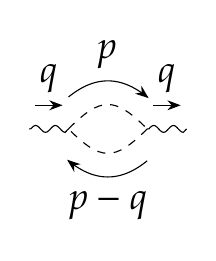
\begin{tikzpicture}
        \begin{feynman}
            \vertex (a) at (-1,0);
            \vertex (b) at (-0.5,0);
            \vertex (c) at (0.5,0);
            \vertex (d) at (1,0);

            \draw[photon, momentum=$q$] (a) -- (b);
            \draw[photon, momentum=$q$] (c) -- (d);
            \draw[scalar, momentum=$p$] (b) to[out=45, in=135, looseness=1.5] (c);
            \draw[scalar, momentum=$p - q$] (c) to[out=-135, in=-45, looseness=1.5] (b);
        \end{feynman}
        \end{tikzpicture}
    \end{minipage}
    \hfill
    \begin{minipage}{0.32\textwidth}
        \centering
        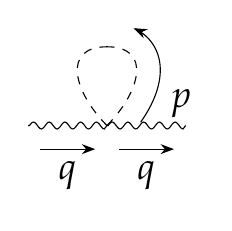
\begin{tikzpicture}
        \begin{feynman}
            \vertex (a) at (-1,0);
            \vertex (b) at (0,0);
            \vertex (c) at (1,0);
            \vertex (d) at (0,1);

            \draw[photon, momentum'=$q$] (a) -- (b);
            \draw[photon, momentum'=$q$] (b) -- (c);
            \draw[scalar, momentum'=$p$] (b) to[out=45, in=0, looseness=1.5] (d);
            \draw[scalar] (b) to[out=135, in=-180, looseness=1.5] (d);
        \end{feynman}
        \end{tikzpicture}
    \end{minipage}
    \hfill
    \begin{minipage}{0.32\textwidth}
        \centering
        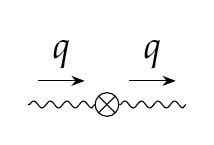
\begin{tikzpicture}
        \begin{feynman}
            \vertex (a) at (-1,0);
            \vertex (b) at (0,0);
            \vertex (c) at (1,0);

            \vertex[counterterm] (b) {};
            
            \draw[photon, momentum=$q$] (a) -- (b);
            \draw[photon, momentum=$q$] (b) -- (c);
        \end{feynman}
        \end{tikzpicture}
    \end{minipage}

    \caption{The three diagrams contributing to the one loop correction of the 1PI photon propegator}
    \label{fig:threephoton}
\end{figure}
\newline
These three diagrams give:
\begin{equation}
\begin{gathered}
    i\mathcal{M}_1 = (-ie)^2\int \frac{d^4 p}{(2\pi)^4} (2p - q)_\mu \frac{i}{p^2 - m^2 + i\epsilon} (2p - q)_\nu \frac{i}{(p - q)^2 - m^2 + i\epsilon} = \\ =
    e^2 \int \frac{d^4 p}{(2\pi)^4} \frac{(2p - q)_\mu(2p - q)_\nu}{\left((p - q)^2 - m^2 + i\epsilon\right)\left(p^2 - m^2 + i\epsilon\right)}
\end{gathered}
\end{equation}
\begin{equation}
    i\mathcal{M}_2 = 2ie^2 \eta_{\mu\nu} \int \frac{d^4 p}{(2\pi)^4} \frac{i}{p^2 - m^2 + i\epsilon} = -2e^2 \int \frac{d^4 p}{(2\pi)^4} \frac{\eta_{\mu\nu}}{p^2 - m^2 + i\epsilon}
\end{equation}
\begin{equation}
    i\mathcal{M}_3 = i\delta_3 \left(\eta_{\mu\nu} q^2 - q_\mu q_\nu\right)
\end{equation}
The third diagram is clear. Let us look at the first two terms give:
\begin{equation}
    e^2 \int \frac{d^4 p}{(2\pi)^4} \left[
        \frac{(2p - q)_\mu(2p - q)_\nu}{\left((p - q)^2 - m^2 + i\epsilon\right)\left(p^2 - m^2 + i\epsilon\right)} - 2 \frac{\eta_{\mu\nu}}{p^2 - m^2 + i\epsilon}
    \right]
\end{equation}
Expanding the nominator in the first term and taking common denominator:
\begin{equation}
    e^2 \int \frac{d^4 p}{(2\pi)^4}
        \frac{4 p_\mu p_\nu - 2(p_\mu q_\nu + q_\mu p_\nu) + q_\mu q_\nu - 2\eta_{\mu\nu} p^2 + 4 \eta_{\mu\nu} pq - 2\eta_{\mu\nu} q^2 + 2\eta_{\mu\nu} m^2}{\left((p - q)^2 - m^2 + i\epsilon\right)\left(p^2 - m^2 + i\epsilon\right)}
\end{equation}
Now we can use Feynman's trick:
\begin{equation}
    A = (p - q)^2 - m^2 + i\epsilon
    \qquad
    B = p^2 - m^2 + i\epsilon
\end{equation}
And this gives:
\begin{equation}
\begin{gathered}
    e^2 \int_0^1 dx \int \frac{d^4 p}{(2\pi)^4}
    \frac{4 p_\mu p_\nu - 2(p_\mu q_\nu + q_\mu p_\nu) + q_\mu q_\nu - 2\eta_{\mu\nu} p^2 + 4 \eta_{\mu\nu} pq - 2\eta_{\mu\nu} q^2 + 2\eta_{\mu\nu} m^2}{\left[
        \left((p - q)^2 - m^2 + i\epsilon\right)x + \left(p^2 - m^2 + i\epsilon\right)(1 - x)
    \right]^2} = \\ =
    e^2 \int_0^1 dx \int \frac{d^4 p}{(2\pi)^4}
    \frac{4 p_\mu p_\nu + q_\mu q_\nu - 2\eta_{\mu\nu} p^2 - 2\eta_{\mu\nu} q^2 + 2\eta_{\mu\nu} m^2}{\left[p^2 - 2qpx + xq^2 - m^2 + i\epsilon\right]^2}
\end{gathered}
\end{equation}
Defining $l = p - qx$, the denominator becomes:
\begin{equation}
\begin{gathered}
    \left[(l + qx)^2 - 2q(l + qx)x + xq^2 - m^2 + i\epsilon\right]^2 = \\ =
    \left[l^2 + x(1 - x)q^2 - m^2 + i\epsilon\right]^2 = \\ =
    \left[l^2 + \Delta\right]^2
\end{gathered}
\end{equation}
Where $\Delta = x(1 - x)q^2 - m^2$. The nominator has four terms that have p-dependence. Since the denominator is now even in $l$, all terms that are odd in $l$ in the nominator vanish, since they create an odd intergrand in an even range:
\begin{equation}
    4p_\mu p_\nu = 4(l + qx)_\mu (l + qx)_\nu = 4l_\mu l_\nu + 4x^2 q_\mu q_\nu + \text{odd terms}
\end{equation}
\begin{equation}
    2(p_\mu q_\nu + q_\mu p_\nu) = 2((l + qx)_\mu q_\nu + q_\mu (l + qx)_\nu) = 4x q_\mu q_\nu + \text{odd terms}
\end{equation}
\begin{equation}
    2\eta_{\mu\nu} p^2 = 2\eta_{\mu\nu} (l + qx)^2 = 2\eta_{\mu\nu} l^2 + 2\eta_{\mu\nu} x^2q^2 + \text{odd terms}
\end{equation}
\begin{equation}
    4\eta_{\mu\nu}qp = 4\eta_{\mu\nu}q(l + qx) = 4x\eta_{\mu\nu}q^2 + \text{odd terms} 
\end{equation}
Putting all of this together gives:
\begin{equation}
\begin{gathered}
    e^2 \int_0^1 dx \int \frac{d^4 l}{(2\pi)^4}
    \frac{4 l_\mu l_\nu + (2x^2 - 4x + 1)q_\mu q_\nu - 2\eta_{\mu\nu} l^2 - 2(x^2 - 2x + 1) \eta_{\mu\nu} q^2 + 2\eta_{\mu\nu} m^2}{\left[l^2 + x(1 - x)q^2 - m^2 + i\epsilon\right]^2} = \\ =
    e^2 \int_0^1 dx \int \frac{d^4 l}{(2\pi)^4}
    \frac{4 l_\mu l_\nu + (2x - 1)^2q_\mu q_\nu - 2\eta_{\mu\nu} l^2 - 2(x - 1)^2 \eta_{\mu\nu} q^2 + 2\eta_{\mu\nu} m^2}{\left[l^2 + \Delta\right]^2}
\end{gathered}
\end{equation}
Using $\int l^\mu l^\nu F(l^2)d^dl = \frac{\eta_{\mu\nu}}{d}\int l^2 F(l^2)dl$ and moving to Euclidean space $l^0 = il^0_E$:
\begin{equation}
    i e^2 \int_0^1 dx \int \frac{d^4 l}{(2\pi)^4}
    \frac{\eta_{\mu\nu} l^2 + (2x - 1)^2q_\mu q_\nu - 2\eta_{\mu\nu} l^2 - 2(x - 1)^2 \eta_{\mu\nu} q^2 + 2\eta_{\mu\nu} m^2}{\left[l^2 + \Delta\right]^2}
\end{equation}
Gathering by order of $l$:
\begin{equation}
    i e^2 \int_0^1 dx \int \frac{d^4 l}{(2\pi)^4}
    \frac{(2x - 1)^2q_\mu q_\nu - 2(x - 1)^2 \eta_{\mu\nu} q^2 + 2\eta_{\mu\nu} m^2}{\left[l^2 + \Delta\right]^2} - \frac{\eta_{\mu\nu} l^2}{\left[l^2 + \Delta\right]^2}
\end{equation}
This is divergent, so we must use dimensional regularization. Taking the intergral to $d = 4 - \epsilon$:
\begin{equation}
\begin{gathered}
    i e^2 \int_0^1 dx \int \frac{d^d l}{(2\pi)^d}
    \frac{(2x - 1)^2q_\mu q_\nu - 2(x - 1)^2 \eta_{\mu\nu} q^2 + 2\eta_{\mu\nu} m^2}{\left[l^2 + \Delta\right]^2} - \frac{\eta_{\mu\nu} l^2}{\left[l^2 + \Delta\right]^2} = \\ =
    \frac{i e^2}{(4\pi)^2} \int_0^1 dx \left[
        \frac{\Gamma\left(\frac{\epsilon}{2}\right)}{\Gamma(2)}\frac{(2x - 1)^2q_\mu q_\nu - 2(x - 1)^2 \eta_{\mu\nu} q^2 + 2\eta_{\mu\nu} m^2}{\Delta^{\frac{\epsilon}{2}}} - \frac{\Gamma(\frac{\epsilon}{2} - 1)}{\Gamma(2)}\frac{2\eta_{\mu\nu}}{\Delta^{\frac{\epsilon}{2}-1}}
    \right] = \\ =
    \frac{i e^2}{(4\pi)^2} \int_0^1 dx \frac{\Gamma\left(\frac{\epsilon}{2}\right)}{\Delta^{\frac{\epsilon}{2}}} \left[
        (2x - 1)^2q_\mu q_\nu - 2(x - 1)^2 \eta_{\mu\nu} q^2 + 2\eta_{\mu\nu} m^2 - \frac{\Gamma(\frac{\epsilon}{2} - 1)}{\Gamma\left(\frac{\epsilon}{2}\right)}2\eta_{\mu\nu} \Delta
    \right]
\end{gathered}
\end{equation}
Using the definition of the Gamma function:
\begin{equation}
    \Gamma\left(\frac{\epsilon}{2}\right) = \left(\frac{\epsilon}{2} - 1\right)\Gamma\left(\frac{\epsilon}{2} - 1\right)
\end{equation}
Then at the limit $\epsilon = 0$, we get:
\begin{equation}
    \frac{\Gamma(\frac{\epsilon}{2} - 1)}{\Gamma\left(\frac{\epsilon}{2}\right)} = \frac{1}{\frac{\epsilon}{2} - 1} \rightarrow -1
\end{equation}
Which means that the last term becomes:
\begin{equation}
     - \frac{\Gamma(\frac{\epsilon}{2} - 1)}{\Gamma\left(\frac{\epsilon}{2}\right)}2\eta_{\mu\nu} \Delta \rightarrow 2\eta_{\mu\nu}x(1 - x)q^2 - 2\eta_{\mu\nu}m^2
\end{equation}
This cancels out with the mass term, leaving:
\begin{equation}
\begin{gathered}
    \frac{i e^2}{(4\pi)^2} \int_0^1 dx \frac{\Gamma\left(\frac{\epsilon}{2}\right)}{\Delta^{\frac{\epsilon}{2}}} \left[
        (2x - 1)^2q_\mu q_\nu - 2[(x - 1)^2 - x(1 - x)] \eta_{\mu\nu} q^2
    \right] = \\ =
    \frac{i e^2}{(4\pi)^2} \int_0^1 dx \frac{\Gamma\left(\frac{\epsilon}{2}\right)}{\Delta^{\frac{\epsilon}{2}}} \left[
        (2x - 1)^2q_\mu q_\nu - 2(2x^2 - 3x + 1) \eta_{\mu\nu} q^2
    \right] = \\ =
    \frac{i e^2}{(4\pi)^2} \int_0^1 dx \frac{\Gamma\left(\frac{\epsilon}{2}\right)}{\Delta^{\frac{\epsilon}{2}}} \left[
        (4x^2 + 4x - 1)q_\mu q_\nu - (4x^2 - 6x + 2) \eta_{\mu\nu} q^2
    \right]
\end{gathered}
\end{equation}
Since the denominator is, at the limit $\epsilon \rightarrow 0$, symmetric around $x = \frac{1}{2}$, we can remove any terms in the paranthesses that are antisymmetric at that range. This includes any multiple of $2x - 1$. Specifically, adding $(1 - 2x) \eta_{\mu\nu}q^2$, will turn the second term into:
\begin{equation}
    - (4x^2 - 6x + 2) \eta_{\mu\nu} q^2 + (1 - 2x) \eta_{\mu\nu}q^2 = 
    - (4x^2 - 4x + 1) \eta_{\mu\nu}q^2
\end{equation}
Exactly like the first term. We can then pull the x-independent factors out of the integral to get:
\begin{equation}
    \frac{i e^2}{(4\pi)^2} \left(q_\mu q_\nu - \eta_{\mu\nu}q^2\right) \int_0^1 dx \frac{\Gamma\left(\frac{\epsilon}{2}\right)}{\Delta^{\frac{\epsilon}{2}}}(4x^2 + 4x - 1)
\end{equation}
And after openning the $Gamma$ function in Lorent expansion:
\begin{equation}
    \frac{i e^2}{(4\pi)^2} \left(q_\mu q_\nu - \eta_{\mu\nu}q^2\right) \int_0^1 dx \left(\frac{2}{\epsilon} - \gamma - \ln \frac{m^2 + x(1 - x)q^2}{4\pi} + O(\epsilon)\right)(2x - 1)^2
\end{equation}
Now, we can finally add the third diagram contribution, which sum up to $-i\Pi_{\mu\nu}$. So, after multiplying by $i$, we get:
\begin{equation}
    \Pi_{\mu\nu}(q) = (\eta_{\mu\nu}q^2 - q_{\mu}q_{\nu})\left(
        \delta_3 + \frac{e^2}{(4\pi)^2} \int_0^1 dx \left(\frac{2}{\epsilon} - \gamma - \ln \frac{m^2 + x(1 - x)q^2}{4\pi} + O(\epsilon)\right)(2x - 1)^2
    \right)
\end{equation}
Which is the form required:
\begin{equation}
    \Pi_{\mu\nu}(q) = (\eta_{\mu\nu}q^2 - q_{\mu}q_{\nu})\Pi(q^2)
\end{equation}
With
\begin{equation}
    \Pi(q^2) = \delta_3 + \frac{e^2}{(4\pi)^2} \int_0^1 dx \left(\frac{2}{\epsilon} - \gamma - \ln \frac{m^2 + x(1 - x)q^2}{4\pi} + O(\epsilon)\right)(2x - 1)^2
\end{equation}
Now, using the renormalization condition $\Pi(M^2) = 0$ for some scale $M$, we get:
\begin{equation}
    \delta_3 = \frac{e^2}{(4\pi)^2} \int_0^1 dx \left(\gamma + \ln \frac{m^2 + x(1 - x)M^2}{4\pi} + O(\epsilon) - \frac{2}{\epsilon}\right)(2x - 1)^2
\end{equation}
So:
\begin{equation}
    \Pi(q^2) = \frac{e^2}{(4\pi)^2} \int_0^1 dx (2x - 1)^2 \ln \frac{m^2 + x(1 - x)M^2}{m^2 + x(1 - x)q^2}
\end{equation}
And when $M^2 \gg m^2$:
\begin{equation}
    \frac{m^2 + x(1 - x)M^2}{m^2 + x(1 - x)q^2} \rightarrow \frac{x(1 - x)M^2}{x(1 - x)q^2} = \frac{M^2}{q^2}
\end{equation}
Which gives:
\begin{equation}
    \Pi(q^2) = \frac{e^2M^2}{(4\pi)^2q^2} \int_0^1 dx (2x - 1)^2
\end{equation}
\begin{equation}
    \Pi(q^2) = \frac{e^2M^2}{3(4\pi)^2q^2}
\end{equation}
\subsection{The beta function revisited}
Now that we have an expression for $\delta_3$, we can plug it into the beta function we got. Taking the derivative:
\begin{equation}
\begin{gathered}
    \frac{d \delta_3}{dM} = \frac{d}{dM} \frac{e^2}{(4\pi)^2}\int_0^1 dx \left(\gamma + \ln \frac{m^2 + x(1 - x)M^2}{4\pi} + O(\epsilon) - \frac{2}{\epsilon}\right)(2x - 1)^2
    = \\ = \frac{e^2}{(4\pi)^2}\int_0^1 dx (2x - 1)^2 \frac{d}{dM}\ln(m^2 + x(1 - x)M^2)
    = \\ = \frac{e^2}{(4\pi)^2}\int_0^1 dx (2x - 1)^2 \frac{2x(1 - x)M}{m^2 + x(1 - x)M^2}
\end{gathered}
\end{equation}
For $M^2 \gg m^2$:
\begin{equation}
\begin{gathered}
    \frac{d \delta_3}{dM} = \frac{e^2}{(4\pi)^2}\int_0^1 dx (2x - 1)^2 \frac{2x(1 - x)M}{x(1 - x)M^2} = \\ =
    \frac{e^2}{(4\pi)^2}\frac{2}{M}\int_0^1 dx (2x - 1)^2 = 
    \frac{2e^2}{3(4\pi)^2}M^{-1}
\end{gathered}
\end{equation}
Which means the $beta$ function is:
\begin{equation}
    \beta = \frac{1}{2}Me \frac{d\delta_3}{dM} =
    \frac{e^3}{3(4\pi)^2}
\end{equation}
The beta function is constant and positive, so we conclude that the coupling grows at high energies (small distances).
\subsection{Generalizing to multiple fields}
Given $N_s$ complex scalar fields and $N_f$ fermion fields, we can look at the one loop correction to the 1PI photon propegator. Each field contributes and additional diagrams as we saw here and in class - every fermion field add a 2 vertices loop with 3 point interactions, and every scalar field adds both a 2 vertices loop with 3 point interactions and a 1 vertex loop with 4 point interaction. These interaction will add similar to how we saw them here, resulting in $\delta_3$ being equal to their total sum. From the linearity of the derivative, we can concluse that the beta function will also be simply the sum of beta functions from each term:
\begin{equation}
    \beta = N_s \frac{e^3}{3(4\pi)^2} + N_f \frac{e^3}{12\pi^2} = \frac{e^3}{48\pi^2}\left(N_s + 4 N_f\right)
\end{equation}

\newpage
\section{The Ward-Takahashi identity in scalar QED}
\subsection{Proving the identity}
Starting from the conservation of the current$\partial_\mu J^\mu = 0$, we know that:
\begin{equation}
    \langle
        \partial_\mu J^\mu(x) \theta_1(x_1) \cdots \theta_n(x_n)
    \rangle =
    -i\sum_{j=1}^n \delta(x - x_j) \langle
         \theta_1(x_1) \cdots \Delta\theta_j(x_j) \cdots \theta_n(x_n)
    \rangle
\end{equation}
Where $\delta \theta_j = \alpha \Delta\theta_j$ for every $1 \le j \le n$.
It's clear then, that in scalar QED, with the symmetry $\phi \rightarrow e^{ie\alpha}\phi$, we can write:
\begin{equation}
    \Delta \phi = ie \phi
    \qquad
    \Delta \phi^\dagger = -ie \phi^\dagger
\end{equation}
And then:
\begin{equation}
    \langle
        \partial_\mu J^\mu(y) \phi^\dagger(x) \phi(0)
    \rangle =
    -i\left[
        \delta(y - x) \langle
            -ie\phi^\dagger(x)\phi(0)
        \rangle +
        \delta(y) \langle
            ie\phi^\dagger(x)\phi(0)
        \rangle 
    \right]
\end{equation}
And Fourier transofrming it gives, for the LHS:
\begin{equation}
\begin{gathered}
    \int d^4x d^4y e^{i(q\cdot y + p \cdot x)}\langle
        (\partial_\mu J^\mu(y)) \phi^\dagger(x) \phi(0)
    \rangle = \\ =
    \left[y\text{ boundary terms}\right] - \int d^4x d^4y \partial_\mu\left(e^{iq\cdot y}\right)e^{ip \cdot x}\langle
        J^\mu(y) \phi^\dagger(x) \phi(0)
    \rangle = \\ =
    -iq_\mu \int d^4x d^4y e^{i(q\cdot y + p \cdot x)}\langle
        J^\mu(y) \phi^\dagger(x) \phi(0)
    \rangle = \\ =
    -iq_\mu W_3^\mu(q, p)
\end{gathered}
\end{equation}
And for the RHS:
\begin{equation}
\begin{gathered}
    i\int d^4x d^4y e^{i(q\cdot y + p \cdot x)}\left[
        \delta(y - x) \langle
            -ie\phi^\dagger(x)\phi(0)
        \rangle +
        \delta(y) \langle
            ie \phi^\dagger(x)\phi(0)
        \rangle 
    \right] = \\ =
    e\int d^4x\left[
        e^{i(q + p) \cdot x} \langle
            \phi^\dagger(x)\phi(0)
        \rangle -
        e^{ip \cdot x} \langle
            \phi^\dagger(x)\phi(0)
        \rangle 
    \right] = \\ =
    e\left[W_2(p + q) - W_2(p)\right]
\end{gathered}
\end{equation}
Giving, as expected:
\begin{equation}
    -iq_\mu W_3^\mu(q, p) = e\left[W_2(p + q) - W_2(p)\right]
\end{equation}
\subsection{Computing in order $e$}
For $y^0 > x^0 > 0$, at order $e$, no loop correction enter the RHS and we get:
\begin{equation}
    e\left[W_2(p + q) - W_2(p)\right] = e\left[\frac{i}{(p + q)^2 - m^2 - i\epsilon} - \frac{i}{p^2 - m^2 - i\epsilon}\right]
\end{equation}
In the LHS, only the first term from the definition of $J^\mu$ remains:
\begin{equation}
\begin{gathered}
    -iq_\mu W_3^\mu(q, p) = \\ =
    -e q_\mu \int d^4x d^4y e^{i(q\cdot y + p \cdot x)}\langle
        \left[
            \phi^\dagger(y) \partial^\mu \phi(y) - (\partial^\mu \phi^\dagger(y))\phi(y)
        \right] \phi^\dagger(x) \phi(0)
    \rangle
\end{gathered}
\end{equation}
There are two terms, the treatment of which is very similar. Starting from the first term
\begin{equation}
    \int d^4x d^4y e^{i(q\cdot y + p \cdot x)}
    \langle
        \phi^\dagger(y) \partial^\mu \phi(y) \phi^\dagger(x) \phi(0)
    \rangle
\end{equation}
Using an inverse Fourier transform for the scalar fields:
\begin{equation}
    \phi(x) = \int \frac{d^4p}{(2\pi)^4}e^{-ipx} \phi(p)
    \qquad
    \partial^\mu \phi(x) = -i \int \frac{d^4p}{(2\pi)^4} e^{-ipx} p^\mu \phi(p)
\end{equation}
\begin{equation}
    \phi^\dagger(x) = \int \frac{d^4p}{(2\pi)^4}e^{ipx} \phi^\dagger(p)
    \qquad
    \partial^\mu \phi^\dagger(x) = i \int \frac{d^4p}{(2\pi)^4} e^{ipx} p^\mu \phi^\dagger(p)
\end{equation}
Gives:
\begin{equation}
\begin{gathered}
    -i\int d^4x d^4y \frac{d^4p_1}{(2\pi)^4} \frac{d^4p_2}{(2\pi)^4} \frac{d^4p_3}{(2\pi)^4} \frac{d^4p_4}{(2\pi)^4} \times \\ \times
    e^{i(q\cdot y + p \cdot x + p_1 y - p_2 y + p_3 x)}
    p_2^\mu
    \langle
        \phi^\dagger(p_1) \phi(p_2) \phi^\dagger(p_3) \phi(p_4)
    \rangle = \\ =
    -i\int \frac{d^4p_1}{(2\pi)^4} \frac{d^4p_2}{(2\pi)^4} \frac{d^4p_3}{(2\pi)^4} \frac{d^4p_4}{(2\pi)^4}
    \delta(p + p_3)
    \delta(q + p_1 - p_2)
    p_2^\mu
    \langle
        \phi^\dagger(p_1) \partial^\mu \phi(p_2) \phi^\dagger(p_3) \phi(p_4)
    \rangle = \\ =
    -i \int \frac{d^4p_1}{(2\pi)^4} \frac{d^4p_4}{(2\pi)^4}
    (q + p_1)^\mu
    \langle
        \phi^\dagger(p_1) \partial^\mu \phi(q + p_1) \phi^\dagger(-p) \phi(p_4)
    \rangle
\end{gathered}
\end{equation}
Similarly, the second term becomes:
\begin{equation}
\begin{gathered}
    i\int d^4x d^4y \frac{d^4p_1}{(2\pi)^4} \frac{d^4p_2}{(2\pi)^4} \frac{d^4p_3}{(2\pi)^4} \frac{d^4p_4}{(2\pi)^4} \times \\ \times
    e^{i(q\cdot y + p \cdot x + p_1 y - p_2 y + p_3 x)}
    p_1^\mu
    \langle
        \phi^\dagger(p_1) \phi(p_2) \phi^\dagger(p_3) \phi(p_4)
    \rangle = \\ =
    i\int \frac{d^4p_1}{(2\pi)^4} \frac{d^4p_4}{(2\pi)^4}
    p_1^\mu
    \langle
        \phi^\dagger(p_1) \phi(q + p_1) \phi^\dagger(-p) \phi(p_4)
    \rangle
\end{gathered}
\end{equation}
Which, in total, gives (renaming $p_1 \rightarrow k, p_4 \rightarrow k'$):
\begin{equation}
    -i q_\mu W_3^\mu (q, p) = i e q_\mu \int \frac{d^4kd^4k'}{(2\pi)^8} \left(q + 2k\right)^\mu
    \langle
        \phi^\dagger(k) \phi(q + k) \phi^\dagger(-p) \phi(k')
    \rangle
\end{equation}
From Wick's theorem, the momentum space four point correlation function gives (similar to correlation function in free theory):
\begin{equation}
\begin{gathered}
    \langle
        \phi^\dagger(k) \phi(q + k) \phi^\dagger(-p) \phi(k')
    \rangle = \\ =
    (2\pi)^8 \Bigg[
        \delta(-q)\delta(-p - k')\frac{i}{k^2 - m^2 + i\epsilon}\frac{i}{p^2 - m^2 + i\epsilon} + \\ +
        \delta(k - k')\delta(k + q + p)\frac{i}{k^2 - m^2 + i\epsilon}\frac{i}{(q + k)^2 - m^2 + i\epsilon}
    \Bigg]
\end{gathered}
\end{equation}
Now, we can place that in the integral and integrate using the delta functions. The first term vanishes for non zero $q$, which means it must vanish identically to be Lorentz invariant. This leaves:
\begin{equation}
    -i q_\mu W_3^\mu (q, p) = i e q_\mu \frac{-(2p + q)^\mu}{((p + q)^2 - m^2 + i\epsilon)(p^2 - m^2 + i\epsilon)}
\end{equation}
The fraction can be split:
\begin{equation}
\begin{gathered}
    \frac{q^2 + 2pq}{((p + q)^2 - m^2 + i\epsilon)(p^2 - m^2 + i\epsilon)} =
    \frac{q^2 + 2pq + p^2 - m^2 - p^2 + m^2}{((p + q)^2 - m^2 + i\epsilon)(p^2 - m^2 + i\epsilon)} = \\ =
    \frac{1}{p^2 - m^2 + i\epsilon} - \frac{1}{(p + q)^2 - m^2 + i\epsilon}
\end{gathered}
\end{equation}
\begin{equation}
    -i q_\mu W_3^\mu (q, p) = e\left[\frac{i}{(p + q)^2 - m^2 + i\epsilon} - \frac{i}{p^2 - m^2 + i\epsilon}\right]
\end{equation}
\subsection{Diagrams contributing to $W_3$ in order $e^3$}
Writing the correlation function in $W_3$ fully:
\begin{equation}
\begin{gathered}
    \langle J^\mu(y)\phi^\dagger(x)\phi(0) \rangle = \\ =
    -ie \langle\left[\phi^\dagger(y)(\partial^\mu\phi(y)) - (\partial_\mu\phi^\dagger(y))\phi(y)\right] \phi^\dagger(x)\phi(0) \rangle +
    2e^2\langle A^\mu(y)\phi^\dagger(y)\phi(y)\phi^\dagger(x)\phi(0) \rangle
\end{gathered}
\end{equation}
This is actually the sum of two types of correlation functions: the scalar four point correlation function, and the scalar four point correlation function plus a photon.
\newline
The first term is just the scalar four point correlation function, but with two of the points being the same point spatially $y$. The diagrams matching this includes the sinlge free theory diagram without a tadpole structure, and its one vertex and two vertices extensions.
\begin{figure}[ht]
    \centering

    \begin{minipage}{0.24\textwidth}
        \centering
        \begin{tikzpicture}
        \begin{feynman}
            \vertex (0) at (-1,0) {0};
            \vertex (y) at (0,0) {y};
            \vertex (x) at (1,0) {x};

            \draw[scalar] (0) -- (y);
            \draw[scalar] (y) -- (x);
        \end{feynman}
        \end{tikzpicture}
    \end{minipage}
    \begin{minipage}{0.24\textwidth}
        \centering
        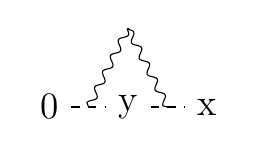
\begin{tikzpicture}
        \begin{feynman}
            \vertex (0) at (-1,0) {0};
            \vertex (y) at (0,0) {y};
            \vertex (x) at (1,0) {x};
            \vertex (1) at (0, 1);
            \vertex (2) at (-0.5, 0);
            \vertex (3) at (0.5, 0);

            \draw[scalar] (0) -- (y);
            \draw[scalar] (y) -- (x);
            \draw[photon] (1) -- (2);
            \draw[photon] (1) -- (3);
        \end{feynman}
        \end{tikzpicture}
    \end{minipage}
    \begin{minipage}{0.24\textwidth}
        \centering
        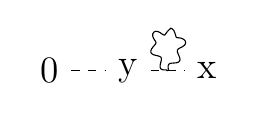
\begin{tikzpicture}
        \begin{feynman}
            \vertex (0) at (-1,0) {0};
            \vertex (y) at (0,0) {y};
            \vertex (x) at (1,0) {x};
            \vertex (1) at (0.5, 0);
            \vertex (v) at (0.5, 0.5);

            \draw[scalar] (0) -- (y);
            \draw[scalar] (y) -- (x);
            \draw[photon] (1) to[out=45, in=0, looseness=1.5] (v);
            \draw[photon] (1) to[out=135, in=180, looseness=1.5] (v);
        \end{feynman}
        \end{tikzpicture}
    \end{minipage}
    \begin{minipage}{0.24\textwidth}
        \centering
        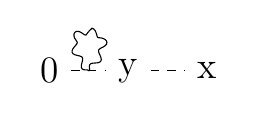
\begin{tikzpicture}
        \begin{feynman}
            \vertex (0) at (-1,0) {0};
            \vertex (y) at (0,0) {y};
            \vertex (x) at (1,0) {x};
            \vertex (1) at (-0.5, 0);
            \vertex (v) at (-0.5, 0.5);

            \draw[scalar] (0) -- (y);
            \draw[scalar] (y) -- (x);
            \draw[photon] (1) to[out=45, in=0, looseness=1.5] (v);
            \draw[photon] (1) to[out=135, in=180, looseness=1.5] (v);
        \end{feynman}
        \end{tikzpicture}
    \end{minipage}
    \begin{minipage}{0.24\textwidth}
        \centering
        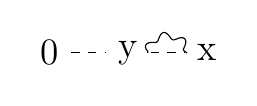
\begin{tikzpicture}
        \begin{feynman}
            \vertex (0) at (-1,0) {0};
            \vertex (y) at (0,0) {y};
            \vertex (x) at (1,0) {x};
            \vertex (1) at (0.25, 0);
            \vertex (2) at (0.75, 0);

            \draw[scalar] (0) -- (y);
            \draw[scalar] (y) -- (x);
            \draw[photon] (1) to[out=90, in=90, looseness=1.5] (2);
        \end{feynman}
        \end{tikzpicture}
    \end{minipage}
    \begin{minipage}{0.24\textwidth}
        \centering
        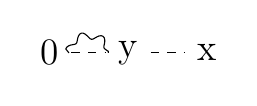
\begin{tikzpicture}
        \begin{feynman}
            \vertex (0) at (-1,0) {0};
            \vertex (y) at (0,0) {y};
            \vertex (x) at (1,0) {x};
            \vertex (1) at (-0.25, 0);
            \vertex (2) at (-0.75, 0);

            \draw[scalar] (0) -- (y);
            \draw[scalar] (y) -- (x);
            \draw[photon] (1) to[out=90, in=90, looseness=1.5] (2);
        \end{feynman}
        \end{tikzpicture}
    \end{minipage}

    \caption{The free propegator and its extensions. The extensions are all of order $e^2$, reaching $e^3$ with the factor from the $W_3$ definition. Additionaly, in every place where there is a two photon vertex there can also be two single photon vertices.}
\end{figure}
\newline
All diagrams for the first term must have an even number of photons, since it has no photons. The second term, however, needs an odd number of photons. In order $e^3$, the only vertex allows is the single photon vertex.
\begin{figure}[ht]
    \centering

    \begin{minipage}{0.24\textwidth}
        \centering
        \begin{tikzpicture}
        \begin{feynman}
            \vertex (0) at (-1.5,0) {0};
            \vertex (y) at (0.5,0) {y};
            \vertex (x) at (1.5,0) {x};
            \vertex (v) at (-0.5,0);

            \draw[scalar] (0) -- (v);
            \draw[photon] (v) to[out=90, in=90, looseness=1.5] (y);
            \draw[scalar] (v) -- (y);
            \draw[scalar] (y) -- (x);
        \end{feynman}
        \end{tikzpicture}
    \end{minipage}
    \begin{minipage}{0.24\textwidth}
        \centering
        \begin{tikzpicture}
        \begin{feynman}
            \vertex (0) at (-1.5,0) {0};
            \vertex (y) at (-0.5,0) {y};
            \vertex (x) at (1.5,0) {x};
            \vertex (v) at (0.5,0);

            \draw[scalar] (0) -- (v);
            \draw[photon] (v) to[out=90, in=90, looseness=1.5] (y);
            \draw[scalar] (v) -- (y);
            \draw[scalar] (y) -- (x);
        \end{feynman}
        \end{tikzpicture}
    \end{minipage}

    \caption{The two diagrams contributing to the second term in order $e^3$.}
\end{figure}
\subsection{Diagrams contributing to $W_2$ in order $e^2$}
On the RHS of the equation, we have a factor $e$, and thus to get the same order, we need to look at diagrams contributing to $W_2$ at order $e^2$. Since $W_2$ is just the scalar propegator, it includes the free propegator, and its one loop extensions.
\begin{figure}[ht]
    \centering

    \begin{minipage}{0.24\textwidth}
        \centering
        \begin{tikzpicture}
        \begin{feynman}
            \vertex (0) at (-1.5,0) {0};
            \vertex (x) at (1.5,0) {x};

            \draw[scalar] (0) -- (x);
        \end{feynman}
        \end{tikzpicture}
    \end{minipage}
    \begin{minipage}{0.24\textwidth}
        \centering
        \begin{tikzpicture}
        \begin{feynman}
            \vertex (0) at (-1.5,0) {0};
            \vertex (y) at (0.5,0);
            \vertex (x) at (1.5,0) {x};
            \vertex (v) at (-0.5,0);

            \draw[scalar] (0) -- (v);
            \draw[photon] (v) to[out=90, in=90, looseness=1.5] (y);
            \draw[scalar] (v) -- (y);
            \draw[scalar] (y) -- (x);
        \end{feynman}
        \end{tikzpicture}
    \end{minipage}
    \begin{minipage}{0.24\textwidth}
        \centering
        \begin{tikzpicture}
        \begin{feynman}
            \vertex (0) at (-1.5,0) {0};
            \vertex (y) at (0,0);
            \vertex (x) at (1.5,0) {x};
            \vertex (v) at (0,0.5);

            \draw[scalar] (0) -- (x);
            \draw[photon] (y) to[out=45, in=0, looseness=1.5] (v);
            \draw[photon] (y) to[out=135, in=180, looseness=1.5] (v);
        \end{feynman}
        \end{tikzpicture}
    \end{minipage}

    \caption{The diagrams contributes to the RHS of the equation.}
\end{figure}
\end{document}
